\documentclass[aps,pra,amsmath,twocolumn,amssymb,superscriptaddress]{revtex4-1}
%=============================================================================
% BEGIN UNFORGIVABLE HACKS
%=============================================================================

\makeatletter
\def\@bibdataout@aps{%
 \immediate\write\@bibdataout{%
  @CONTROL{%
   apsrev41Control,author="08",editor="1",pages="0",title="0",year="1",eprint="1"%
  }%
 }%
 \if@filesw
  \immediate\write\@auxout{\string\citation{apsrev41Control}}%
 \fi
}%
\makeatother % Phew.

%=============================================================================
% END UNFORGIVABLE HACKS
%=============================================================================

\usepackage{amssymb}
\usepackage{amsthm}
\usepackage{amsfonts}
\usepackage{complexity}
\usepackage{graphicx}% Include figure files
\usepackage{dcolumn}% Align table columns on decimal point
\usepackage{bm}% bold math
\usepackage{hyperref}
\usepackage{enumerate}
\usepackage{algorithm}
\usepackage{algpseudocode}
    \renewcommand{\algorithmicrequire}{\textbf{Input:}}
    \renewcommand{\algorithmicensure}{\textbf{Output:}}
    \newcommand{\inlinecomment}[1]{\Comment {\footnotesize #1} \normalsize}
    \newcommand{\linecomment}[1]{\State \(\triangleright\) {\footnotesize #1} \normalsize}
    %\renewcommand{\algorithmiccomment}[1]{\State\(\triangleright\) #1}
    
\usepackage{multirow}

\newtheorem{theorem}{Theorem}
\newtheorem{lemma}{Lemma}
\newtheorem{definition}{Definition}
\newtheorem{corollary}{Corollary}

%    Q-circuit version 2
%    Copyright (C) 2004  Steve Flammia & Bryan Eastin
%    Last modified on: 9/16/2011
%
%    This program is free software; you can redistribute it and/or modify
%    it under the terms of the GNU General Public License as published by
%    the Free Software Foundation; either version 2 of the License, or
%    (at your option) any later version.
%
%    This program is distributed in the hope that it will be useful,
%    but WITHOUT ANY WARRANTY; without even the implied warranty of
%    MERCHANTABILITY or FITNESS FOR A PARTICULAR PURPOSE.  See the
%    GNU General Public License for more details.
%
%    You should have received a copy of the GNU General Public License
%    along with this program; if not, write to the Free Software
%    Foundation, Inc., 59 Temple Place, Suite 330, Boston, MA  02111-1307  USA

% Thanks to the Xy-pic guys, Kristoffer H Rose, Ross Moore, and Daniel Müllner,
% for their help in making Qcircuit work with Xy-pic version 3.8.  
% Thanks also to Dave Clader, Andrew Childs, Rafael Possignolo, Tyson Williams,
% Sergio Boixo, Cris Moore, Jonas Anderson, and Stephan Mertens for helping us test 
% and/or develop the new version.

\usepackage[color]{xy}
\UseCrayolaColors
\xyoption{matrix}
\xyoption{frame}
\xyoption{arrow}
\xyoption{arc}

\usepackage{ifpdf}
\ifpdf
\else
\PackageWarningNoLine{Qcircuit}{Qcircuit is loading in Postscript mode.  The Xy-pic options ps and dvips will be loaded.  If you wish to use other Postscript drivers for Xy-pic, you must modify the code in Qcircuit.tex}
%    The following options load the drivers most commonly required to
%    get proper Postscript output from Xy-pic.  Should these fail to work,
%    try replacing the following two lines with some of the other options
%    given in the Xy-pic reference manual.
\xyoption{ps}
\xyoption{dvips}
\fi

% The following resets Xy-pic matrix alignment to the pre-3.8 default, as
% required by Qcircuit.
\entrymodifiers={!C\entrybox}

%\newcommand{\bra}[1]{{\left\langle{#1}\right\vert}}
%\newcommand{\ket}[1]{{\left\vert{#1}\right\rangle}}
    % Defines Dirac notation. %7/5/07 added extra braces so that the commands will work in subscripts.
\newcommand{\qw}[1][-1]{\ar @{-} [0,#1]}
\newcommand{\eqw}[1][-1]{\ar @{-} @[Red] [0,#1]}
    % Defines a wire that connects horizontally.  By default it connects to the object on the left of the current object.
    % WARNING: Wire commands must appear after the gate in any given entry.
\newcommand{\qwx}[1][-1]{\ar @{-} [#1,0]}
    % Defines a wire that connects vertically.  By default it connects to the object above the current object.
    % WARNING: Wire commands must appear after the gate in any given entry.
\newcommand{\cw}[1][-1]{\ar @{=} [0,#1]}
    % Defines a classical wire that connects horizontally.  By default it connects to the object on the left of the current object.
    % WARNING: Wire commands must appear after the gate in any given entry.
\newcommand{\cwx}[1][-1]{\ar @{=} [#1,0]}
    % Defines a classical wire that connects vertically.  By default it connects to the object above the current object.
    % WARNING: Wire commands must appear after the gate in any given entry.
\newcommand{\gate}[1]{*+<.6em>{#1} \POS ="i","i"+UR;"i"+UL **\dir{-};"i"+DL **\dir{-};"i"+DR **\dir{-};"i"+UR **\dir{-},"i" \qw}
\newcommand{\eboxgate} [1]{*+<.6em>{#1} \POS ="i","i"+UR;"i"+UL **[red]\dir{-};"i"+DL **[red]\dir{-};"i"+DR **[red]\dir{-};"i"+UR **[red]\dir{-},"i" \eqw}
\newcommand{\circgate}[1]{*+<0.6em>[o][F-]{#1} \eqw}
\newcommand{\ecircgate}[1]{*+<0.6em>[o][F-:red]{#1} \eqw}
\newcommand{\filtergt}[1]{\eboxgate{\scriptscriptstyle{#1}}}
\newcommand{\idealdec}{*+<1.2em>{\phantom{*}} \POS ="i","i"+UL;"i"+DL **[red]\dir{-};"i"+R **[red]\dir{-};"i"+UL **[red]\dir{-},"i" \eqw}

    % Boxes the argument, making a gate.
\newcommand{\meter}{*=<1.8em,1.4em>{\xy ="j","j"-<.778em,.322em>;{"j"+<.778em,-.322em> \ellipse ur,_{}},"j"-<0em,.4em>;p+<.5em,.9em> **\dir{-},"j"+<2.2em,2.2em>*{},"j"-<2.2em,2.2em>*{} \endxy} \POS ="i","i"+UR;"i"+UL **\dir{-};"i"+DL **\dir{-};"i"+DR **\dir{-};"i"+UR **\dir{-},"i" \qw}
    % Inserts a measurement meter.
    % In case you're wondering, the constants .778em and .322em specify
    % one quarter of a circle with radius 1.1em.
    % The points added at + and - <2.2em,2.2em> are there to strech the
    % canvas, ensuring that the size is unaffected by erratic spacing issues
    % with the arc.
\newcommand{\measure}[1]{*+[F-:<.9em>]{#1} \qw}
    % Inserts a measurement bubble with user defined text.
\newcommand{\measuretab}[1]{*{\xy*+<.6em>{#1}="e";"e"+UL;"e"+UR **\dir{-};"e"+DR **\dir{-};"e"+DL **\dir{-};"e"+LC-<.5em,0em> **\dir{-};"e"+UL **\dir{-} \endxy} \qw}
    % Inserts a measurement tab with user defined text.
\newcommand{\measureD}[1]{*{\xy*+=<0em,.1em>{#1}="e";"e"+UR+<0em,.25em>;"e"+UL+<-.5em,.25em> **\dir{-};"e"+DL+<-.5em,-.25em> **\dir{-};"e"+DR+<0em,-.25em> **\dir{-};{"e"+UR+<0em,.25em>\ellipse^{}};"e"+C:,+(0,1)*{} \endxy} \qw}
\newcommand{\emeasureD}[1]{*{\xy*+=<0em,.1em>{#1}="e";"e"+UR+<0em,.25em>;"e"+UL+<-.5em,.25em> **[red]\dir{-};"e"+DL+<-.5em,-.25em> **[red]\dir{-};"e"+DR+<0em,-.25em> **[red]\dir{-};{"e"+UR+<0em,.25em>\ellipse{}};"e"+C:,+(0,1)*{} \endxy} \qw}
    % Inserts a D-shaped measurement gate with user defined text.
\newcommand{\multimeasure}[2]{*+<1em,.9em>{\hphantom{#2}} \qw \POS[0,0].[#1,0];p !C *{#2},p \drop\frm<.9em>{-}}
    % Draws a multiple qubit measurement bubble starting at the current position and spanning #1 additional gates below.
    % #2 gives the label for the gate.
    % You must use an argument of the same width as #2 in \ghost for the wires to connect properly on the lower lines.
\newcommand{\multimeasureD}[2]{*+<1em,.9em>{\hphantom{#2}} \POS [0,0]="i",[0,0].[#1,0]="e",!C *{#2},"e"+UR-<.8em,0em>;"e"+UL **\dir{-};"e"+DL **\dir{-};"e"+DR+<-.8em,0em> **\dir{-};{"e"+DR+<0em,.8em>\ellipse^{}};"e"+UR+<0em,-.8em> **\dir{-};{"e"+UR-<.8em,0em>\ellipse^{}},"i" \qw}
    % Draws a multiple qubit D-shaped measurement gate starting at the current position and spanning #1 additional gates below.
    % #2 gives the label for the gate.
    % You must use an argument of the same width as #2 in \ghost for the wires to connect properly on the lower lines.
\newcommand{\control}{*!<0em,.025em>-=-<.2em>{\bullet}}
    % Inserts an unconnected control.
\newcommand{\controlo}{*+<.01em>{\xy -<.095em>*\xycircle<.19em>{} \endxy}}
    % Inserts a unconnected control-on-0.
\newcommand{\ctrl}[1]{\control \qwx[#1] \qw}
    % Inserts a control and connects it to the object #1 wires below.
\newcommand{\ctrlo}[1]{\controlo \qwx[#1] \qw}
    % Inserts a control-on-0 and connects it to the object #1 wires below.
\newcommand{\targ}{*+<.02em,.02em>{\xy ="i","i"-<.39em,0em>;"i"+<.39em,0em> **\dir{-}, "i"-<0em,.39em>;"i"+<0em,.39em> **\dir{-},"i"*\xycircle<.4em>{} \endxy} \qw}
    % Inserts a CNOT target.
\newcommand{\qswap}{*=<0em>{\times} \qw}
    % Inserts half a swap gate.
    % Must be connected to the other swap with \qwx.
\newcommand{\multigate}[2]{*+<1em,.9em>{\hphantom{#2}} \POS [0,0]="i",[0,0].[#1,0]="e",!C *{#2},"e"+UR;"e"+UL **\dir{-};"e"+DL **\dir{-};"e"+DR **\dir{-};"e"+UR **\dir{-},"i" \qw}
    % Draws a multiple qubit gate starting at the current position and spanning #1 additional gates below.
    % #2 gives the label for the gate.
    % You must use an argument of the same width as #2 in \ghost for the wires to connect properly on the lower lines.
\newcommand{\ghost}[1]{*+<1em,.9em>{\hphantom{#1}} \qw}
    % Leaves space for \multigate on wires other than the one on which \multigate appears.  Without this command wires will cross your gate.
    % #1 should match the second argument in the corresponding \multigate.
\newcommand{\push}[1]{*{#1}}
    % Inserts #1, overriding the default that causes entries to have zero size.  This command takes the place of a gate.
    % Like a gate, it must precede any wire commands.
    % \push is useful for forcing columns apart.
    % NOTE: It might be useful to know that a gate is about 1.3 times the height of its contents.  I.e. \gate{M} is 1.3em tall.
    % WARNING: \push must appear before any wire commands and may not appear in an entry with a gate or label.
\newcommand{\gategroup}[6]{\POS"#1,#2"."#3,#2"."#1,#4"."#3,#4"!C*+<#5>\frm{#6}}
    % Constructs a box or bracket enclosing the square block spanning rows #1-#3 and columns=#2-#4.
    % The block is given a margin #5/2, so #5 should be a valid length.
    % #6 can take the following arguments -- or . or _\} or ^\} or \{ or \} or _) or ^) or ( or ) where the first two options yield dashed and
    % dotted boxes respectively, and the last eight options yield bottom, top, left, and right braces of the curly or normal variety.  See the Xy-pic reference manual for more options.
    % \gategroup can appear at the end of any gate entry, but it's good form to pick either the last entry or one of the corner gates.
    % BUG: \gategroup uses the four corner gates to determine the size of the bounding box.  Other gates may stick out of that box.  See \prop.

\newcommand{\rstick}[1]{*!L!<-.5em,0em>=<0em>{#1}}
    % Centers the left side of #1 in the cell.  Intended for lining up wire labels.  Note that non-gates have default size zero.
\newcommand{\lstick}[1]{*!R!<.5em,0em>=<0em>{#1}}
    % Centers the right side of #1 in the cell.  Intended for lining up wire labels.  Note that non-gates have default size zero.
\newcommand{\ustick}[1]{*!D!<0em,-.5em>=<0em>{#1}}
    % Centers the bottom of #1 in the cell.  Intended for lining up wire labels.  Note that non-gates have default size zero.
\newcommand{\dstick}[1]{*!U!<0em,.5em>=<0em>{#1}}
    % Centers the top of #1 in the cell.  Intended for lining up wire labels.  Note that non-gates have default size zero.
\newcommand{\Qcircuit}{\xymatrix @*=<0em>}
    % Defines \Qcircuit as an \xymatrix with entries of default size 0em.
\newcommand{\link}[2]{\ar @{-} [#1,#2]}
    % Draws a wire or connecting line to the element #1 rows down and #2 columns forward.
\newcommand{\pureghost}[1]{*+<1em,.9em>{\hphantom{#1}}}
    % Same as \ghost except it omits the wire leading to the left. 
%%%%%%%%%%%%%%%%%%%%%%%%%%%%%%%%%%%%%%%%%%%%%%%%%%%%%%%%%%%%%%%%%%%%%%%%%%%%%%%%%%%%%%%%%%
\newcommand{\multiprepareC}[2]{*+<1em,.9em>{\hphantom{#2}}\save[0,0].[#1,0];p\save !C
  *{#2},p+RU+<0em,0em>;+LU+<+.8em,0em> **\dir{-}\restore\save +RD;+RU **\dir{-}\restore\save
  +RD;+LD+<.8em,0em> **\dir{-} \restore\save +LD+<0em,.8em>;+LU-<0em,.8em> **\dir{-} \restore \POS
  !UL*!UL{\cir<.9em>{u_r}};!DL*!DL{\cir<.9em>{l_u}}\restore}
   % Draws a multiple qubit reverse-D-shaped preparation gate starting at the current position and spanning #1 additional gates below.
   % #2 gives the label for the gate.
   % You must use an argument of the same width as #2 in \pureghost for the wires to connect properly on
% the lower lines.
\newcommand{\prepareC}[1]{*{\xy*+=+<.5em>{\vphantom{#1\rule{0em}{.1em}}}*\cir{l^r};p\save*!L{#1} \restore\save+UC;+UC+<.5em,0em>*!L{\hphantom{#1}}+R **\dir{-} \restore\save+DC;+DC+<.5em,0em>*!L{\hphantom{#1}}+R **\dir{-} \restore\POS+UC+<.5em,0em>*!L{\hphantom{#1}}+R;+DC+<.5em,0em>*!L{\hphantom{#1}}+R **\dir{-} \endxy}}
   % Inserts a reverse-D-shaped preparation gate with user defined text.
\newcommand{\poloFantasmaCn}[1]{{{}^{#1}_{\phantom{#1}}}}



\def\ket#1{\left|#1\right\rangle}
\def\bra#1{\langle#1|}
\newcommand{\ketbra}[2]{|#1\rangle\!\langle#2|}
\newcommand{\braket}[2]{\langle#1|#2\rangle}
% \newcommand{\note}[1]{({\bf note: #1})}
\newcommand{\prob}[1]{{\rm Pr}\left(#1 \right)}
% \newcommand{\Tr}[1]{{\rm Tr}\!\left[#1 \right]}
\newcommand{\expect}[2]{{\mathbb{E}_{#2}}\!\left\{#1 \right\}}
\newcommand{\var}[2]{{\mathbb{V}_{#2}}\!\left\{#1 \right\}}
\newcommand{\CRej}{\text{RejF }}

\newcommand{\sinc}{\operatorname{sinc}}
\newcommand{\reset}{\mathrm{reset}}


% fix: supported only for revtex
%\newcommand{\openone}{\mathbb{I}}
% fix: unsupported with iopart
%\newcommand{\eqref}[1]{(\ref{#1})}

\newcommand{\sde}{\mathrm{sde}}
\newcommand{\Z}{\mathbb{Z}}
\newcommand{\RR}{\mathbb{R}}
\newcommand{\w}{\omega}
\newcommand{\Kap}{\kappa}

\newcommand{\Tchar}{$T$}
\newcommand{\T}{\Tchar~}
\newcommand{\TT}{\mathrm{T}}
\newcommand{\ClT}{\{{\rm Clifford}, \Tchar\}~}
\newcommand{\Tcount}{\Tchar--count~}
\newcommand{\Tcountper}{\Tchar--count}
\newcommand{\Tcounts}{\Tchar--counts~}
\newcommand{\Tdepth}{\Tchar--depth~}
\newcommand{\Zr}{\Z[i,1/\sqrt{2}]}
\newcommand{\ve}{\varepsilon}

\newcommand{\eq}[1]{\hyperref[eq:#1]{(\ref*{eq:#1})}}
\renewcommand{\sec}[1]{\hyperref[sec:#1]{Section~\ref*{sec:#1}}}
\newcommand{\app}[1]{\hyperref[app:#1]{Appendix~\ref*{app:#1}}}
%\newcommand{\app}[1]{the supplentary material}
\newcommand{\fig}[1]{\hyperref[fig:#1]{Figure~\ref*{fig:#1}}}
\newcommand{\thm}[1]{\hyperref[thm:#1]{Theorem~\ref*{thm:#1}}}
\newcommand{\lem}[1]{\hyperref[lem:#1]{Lemma~\ref*{lem:#1}}}
\newcommand{\tab}[1]{\hyperref[tab:#1]{Table~\ref*{tab:#1}}}
\newcommand{\cor}[1]{\hyperref[cor:#1]{Corollary~\ref*{cor:#1}}}
\newcommand{\alg}[1]{\hyperref[alg:#1]{Algorithm~\ref*{alg:#1}}}
\newcommand{\defn}[1]{\hyperref[def:#1]{Definition~\ref*{def:#1}}}


\newcommand{\targfix}{\qw {\xy {<0em,0em> \ar @{ - } +<.39em,0em>
\ar @{ - } -<.39em,0em> \ar @{ - } +
<0em,.39em> \ar @{ - }
-<0em,.39em>},<0em,0em>*{\rule{.01em}{.01em}}*+<.8em>\frm{o}
\endxy}}

\newenvironment{proofof}[1]{\begin{trivlist}\item[]{\flushleft\it
Proof of~#1.}}
{\qed\end{trivlist}}


\newcommand{\cu}[1]{{\textcolor{red}{#1}}}
\newcommand{\tout}[1]{{}}
% \newcommand{\beq}{\begin{equation}}
% \newcommand{\eeq}{\end{equation}}
% \newcommand{\beqa}{\begin{eqnarray}}
\newcommand{\good}{{\rm good}}
\newcommand{\bad}{{\rm bad}}
% \newcommand{\eeqa}{\end{eqnarray}}

\newcommand{\id}{\openone}
%\newcommand{\id}{\mathbb{I}}

\newcommand{\etal}{\emph{et al.}}
\newcommand{\ii}{\mathrm{i}}
\newcommand{\ee}{\mathrm{e}}

\hyphenation{FPGA}
\hyphenation{FPGAs}
\hyphenation{RFPE}

%%%%%%%%%%%%%%%%%%%%%%% a bit nicer hypelinks %%%%%%%%%%%%%%%%%%%%%%%%%%%%%

\usepackage[usenames,dvipsnames]{xcolor}
\hypersetup{
    colorlinks=true,       % false: boxed links; true: colored links
    linkcolor=Maroon,          % color of internal links (change box color with linkbordercolor)
    citecolor=OliveGreen,        % color of links to bibliography
    filecolor=magenta,      % color of file links
    urlcolor=Blue           % color of external links
}

%%%%%%%%%%%%%%%%%%%%%%% a bit nicer hypelinks %%%%%%%%%%%%%%%%%%%%%%%%%%%%%

\begin{document}

%=============================================================================
% FRONT MATTER
%=============================================================================

\title{Supplemental material for efficient Bayesian phase estimation}
\author{Nathan Wiebe}
\affiliation{Quantum Architectures and Computation Group, Microsoft Research, Redmond, WA (USA)}

\author{Chris Granade}
\affiliation{Centre for Engineered Quantum Systems, Sydney, NSW (Australia)}
\affiliation{School of Physics, University of Sydney, Sydney, NSW (Australia)}

%\begin{abstract}
   % We provide a new efficient adaptive algorithm for performing phase
    %estimation that does not require that the user infer the bits of the
    %eigenphase in reverse order; rather it directly infers the phase and
    %estimates the uncertainty in the phase directly from experimental data.  It is highly flexible, recovers from failures, and can be run in the
    %presence of decoherence and other experimental imperfections
    %and is as fast or faster than existing methods that are classically efficient.
%\end{abstract}

\maketitle



\onecolumngrid

%=============================================================================
\section{Variance Reduction Strategies}
\label{app:var-reduction}
%=============================================================================

An important drawback of RFPE is  the tails for the distribution of errors in phase estimation can be quite fat in typical applications, meaning that there is significant probability that the error in the inferred eigenphase is orders of magnitude greater than the median.  Such a distribution can be seen in~\fig{PEerrorhist} where we see that although the median error is roughly $10^{-10}$ radians after $100$ updates for $m>50$  a non--negligible fraction of the experiments have error on the order of $1$.    

Fortunately, the need to always repeat the algorithm and use a majority voting scheme to reduce the variance of the estimate is mitigated by the fact that the algorithm outputs $\sigma$ which estimates the uncertainty in the resultant eigenphase. 
Alternatively, less aggressive experiments can be chosen in the guess heuristic or multi--modal models for the prior distribution (such as Gaussian mixture models) can be used.  The later approach can be quite valuable in computer vision and machine learning, however here we have an additional freedom not typically enjoyed in those fields: we can perform adaptive experiments to test to see if our current hypothesis is correct.

The central idea behind our restarting strategy is to examine the decay of $\sigma$ with the number of experiments.  In ideal cases, the error decays exponentially which means that it is easy to see when the algorithm fails by plotting $\sigma$ on a semi--log plot.  Such intuition can be easily automated.  The idea behind our restarting algorithm is to first estimate the derivative of $\log(\sigma)$ with respect to the experiment number and determine whether it is less than a threshold.  If it is less than the threshold, perform an experiment to test to see if the value of $\mu$ that has been learned so far is accurate (as per our incoherent phase estimation algorithm).  If it is found to be innacurate then restart the algorithm and abandon the information learned so far.  The restarting portion of this algorithm is given in~\alg{restart}.

When a restarting strategy like this is employed, we need to modify the model selection criteria.  Previously, we used the value of $\mu$ yielded by the most recent experiment as our estimate.   Given that a restart late in the algorithm can reset all information learned about a model, it makes sense in this context to use the value of $\mu$ corresponding to the smallest $\sigma$ observed.  This corresponds to the model that the inference algorithm has the greatest certainty.

We see in~\fig{restart} that this strategy of restarting substantially reduces the weights of the tails.  In fact, the mean error in the inference falls from $0.0513$ radians to $1.08\times 10^{-6}$ radians.  This shows that this resetting strategy substantially reduce the probability of a large error occuring in the estimate of the eigenphase.  Heuristic error correction methods can therefore be effective at reducing the mean error.  Previous approaches that succeeded in making the mean--error small used costly numerically optimized experiments, which render such approaches impractical for online phase estimation~\cite{granade_robust_2012,ferrie_how_2013, wiebe_hamiltonian_2014,wiebe_quantum_2014-1,WGC15}.

Note that Kitaev's phase estimation algorithm also can have a high probability of failure throughout the algorithm, so one might wonder if these restarting strategies might also be of value for traditional phase estimation algoirthms.  Unfortunately, these strategies cannot be easily translated to Kitaev's PE algorithm because the most expensive experiments are performed first.  Thus, restarting does not allow the algorithm to combat decoherence, nor can it be used to inexpensively fix situations where one of the bits is inferred improperly.

Not all errors occur because of decoherence.  Because rejection filtering is an approximate Bayesian method, one pathology that can occur is that the algorithm fails to learn because the approximate nature of the resampling step may exclude a region of the model space that in fact contains the true model.  This is especially common when the inference algorithm is provided with a datum for which the model that has maximum apriori probability assigns low probability.  In such circumstances rejection filtering can become convinced of a hypotheses that is not true and the algorithm will not continue to learn.  

If the algorithm stops learning then it is seldom advisable to restart the entire algorithm from scratch.  Instead, a better approach is to follow the same strategy considered above by proposing an experiment to test to see if the current uncertainty is less than the true error.  If the test fails then rather than restarting the variance of the model is increased by a constant factor and the inference is continued.  This protocol is taken in~\fig{rms} of the main body wherein the variance is increased by a factor of 100 if the test fails.

\begin{figure*}
    \begin{centering}
        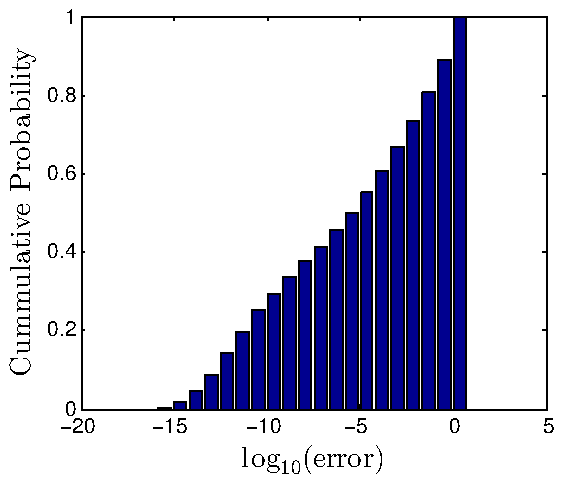
\includegraphics[width=0.3\linewidth]{CProb50.pdf}
        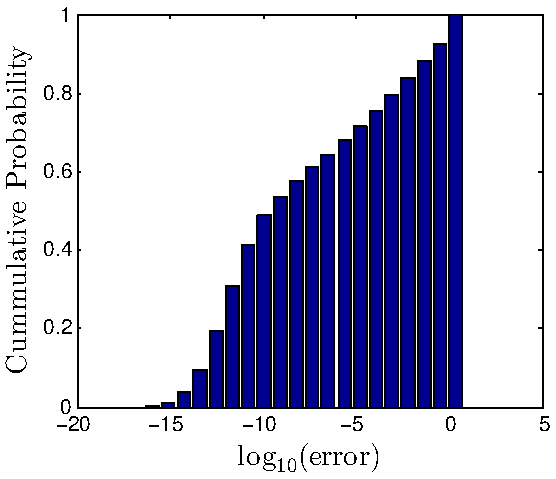
\includegraphics[width=0.3\linewidth]{CProb100.pdf}
        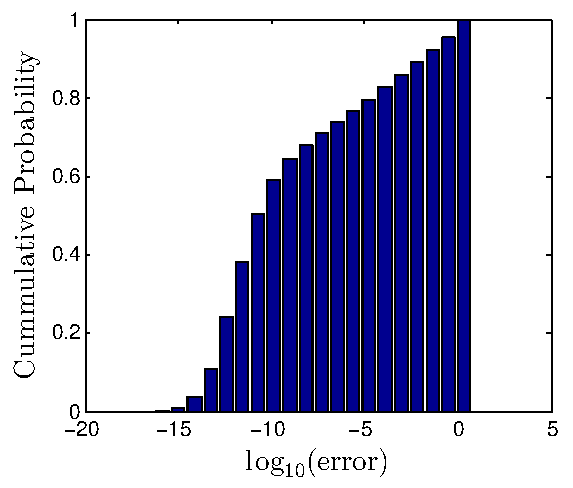
\includegraphics[width=0.3\linewidth]{CProb200.pdf}
    \end{centering}
    \caption{\label{fig:PEerrorhist}
     Cumulative distribution function of probability that PE error is less than $x$ after $150$ updates for $m=50$ (left) $m=100$ (middle) $m=200$ (right).
    }
\end{figure*}

\begin{figure*}
    \begin{centering}
        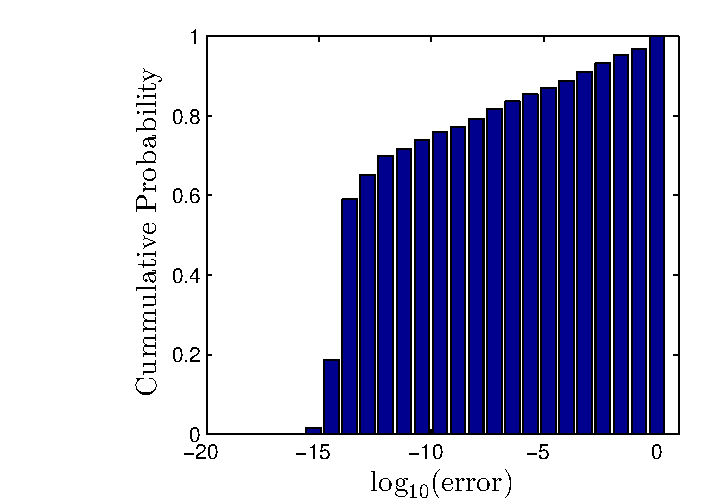
\includegraphics[width=0.35\linewidth]{restartNone.pdf}
        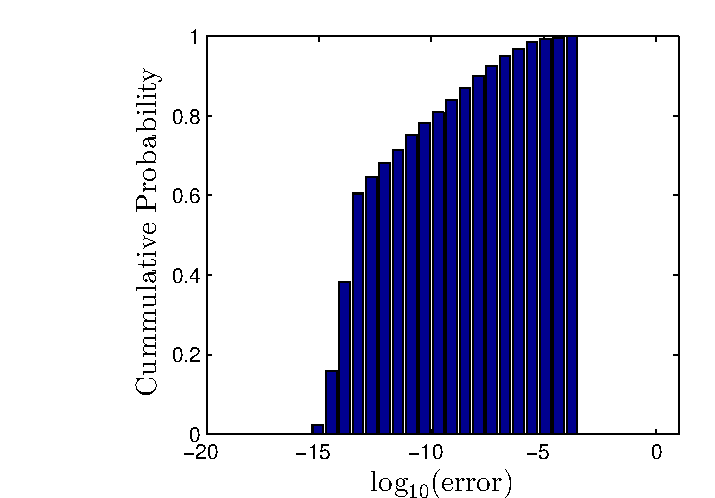
\includegraphics[width=0.35\linewidth]{restartp10.pdf}
    \end{centering}
    \caption{\label{fig:restart}
     Cumulative distribution function of probability that PE error is less than $x$ after $200$ updates for $m=2000$ for $\Gamma=\infty$ (left) $\Gamma=0.1$ (right) and $\tau=0.1$.  Estimate of CDF consists of $1000$ random eigenphase inference problems with $T_2=\infty$.
    }
\end{figure*}

\subsection{Variance reduction in reset rule for decoherant systems}
While the restart rule given in the main body is sufficient to track the eigenstates, it is not optimal because it fails to take into account that previous restarts may contain information about the eigenstate that the estimate is currently focused on.  One way of approaching this problem is to apply the following strategy during the inference process.  

Assume that the spectral gaps are promised to be at least $\Delta$.
After restart, if eigenvalue $\lambda$ is known with uncertainty $\sigma_\lambda$ from a previous restart such that $|\mu-\lambda| \le \sqrt{\sigma^2 + \sigma_\lambda^2}\le \Delta$ then $\mu\gets \lambda$ and $\sigma\gets \sigma_\lambda$ if $\sigma \ge \sigma_\lambda$.  This procedure states that if there is high likelihood that the eigenvalue in question corresponding to one that has been approximately inferred previously, then the current estimate should be set to the previous best known result.  This can lead to a possibility of falsely concluding that the current state actually corresponds to an eigenvalue that has previously been inferred, but that can be addressed by using a more stringent condition on the number of standard deviations (or equivalently on the $p$-value) that the user wishes to use to balance type $1$ versus type $2$ errors for this test.


%=============================================================================
\section{Stability Against Errors in the Likelihood Function}
%=============================================================================


Our algorithm is not only robust against well-known depolarizing noise but is robust against errors in the assumed likelihood function.
That is, by using rejection filtering, we retain the robustness previously shown for particle filtering
in quantum information applications \cite{ferrie_likelihood-free_2014,wiebe_quantum_2014-1,stenberg_efficient_2014}.
We demonstrate this in~\fig{gamma} wherein we introduce depolarizing noise of strength $\gamma$ to our experimental system, but do not include such noise in the likelihood function.  For example, with $\gamma=0.4$, the measurement outcome of phase estimation is replaced with a random bit with probability $40\%$.  Although this may seem qualitatively similar to the numerical examples for depolarizing noise considered in the main body of the paper, this case is much more pathological because it is only used to generate the experimental data and is not permitted in the model of the system used in the likelihood function.  This raises the possibility that the algorithm could become confused due to experimental results that are fundamentally inconsistent with the assumed likelihood function for the system.

\fig{gamma} shows that the inclusion of uncharacterized depolarizing noise does not actually prevent the eigenvalue from being estimated.  Rather it reduces the number of bits per experiment that the algorithm can infer.  We see this by fitting the exponential part of the data in~\fig{gamma} (along with similar data for $\gamma=0.1$, $\gamma=0.3$, $\gamma=0.5$) and find that the error decay exponent, $\lambda$, to shrink as roughly $\lambda \approx 0.17e^{-3.1\gamma}$ it does not prevent our algorithm from learning at an exponential rate (until depolarizing noise becomes significant).  Thus RFPE continue to work even in the presence of depolarizing noise sources that are both strong and uncharacterized.



%=============================================================================
\section{Stability of Rejection Filtering PE}
\label{app:stability}
%=============================================================================

\begin{figure}
    \begin{centering}
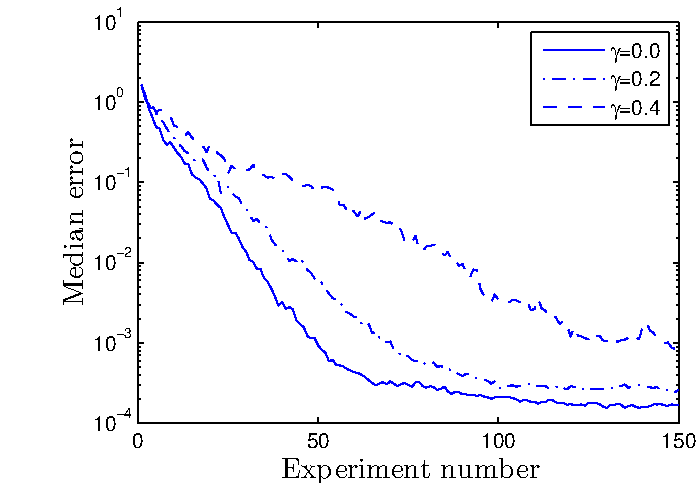
\includegraphics[width=0.45\linewidth]{Gammascale.pdf}
    \end{centering}
    \caption{\label{fig:gamma}
Errors in inference for phase estimation with different levels of un-modeled noise, $\gamma$, for $T_2=1000$.  In each instance the initial state was taken to be a fixed, but unknown, eigenstate of the Hamiltonian.  The median was found for $100$ randomly chosen values of the eigenphase of this fixed initial eigenstate.
    }
\end{figure}

One way in which the rejection sampling algorithm can break down is if the likelihood function becomes too flat relative to the number of discrete samples, $m$, drawn from the prior distribution.  This breakdown occurs because the sample variance in the posterior mean is much greater than the difference between the prior mean and posterior means, which are not expected to be approximately the same if the likelihood function has little variation.  This in effect implies that the dynamics of the mean will essentially be a random walk and as a result we do not expect that our rejection sampling method to perform well if the likelihood function is too flat.  

In practice, the flatness of the distribution can be reduced by batching several experiments together and processing them.  This process is in general inefficient, but can be made efficient if an appropriate value of $\kappa_E$ is known for each datum recoreded.

The question remaining is: how flat is too flat?  We show in the theorem below that if the number of samples taken from the true posterior distribution does not scale at least inverse quadratically with the scale of relative fluctuations in the likelihood function then we expect the posterior variance to be much greater than the shift in the means.  
\begin{theorem}
Assume that for all $j$ $P(E|x_j) =\alpha+\delta_j$ where $|\delta_j|\le \delta$ and $\alpha \ge 10\delta$ and assume that $x_j\sim P(x_j)$.  If we then define $\mu_0 := \sum_{j} P(x_j) x_j$, $\mu_1:= \sum_j P(x_j|E) x_j$ and $\sigma_1^2$ to be the posterior variance then $|\mu_1 - \mu_0| \in \Omega(\sigma_1/\sqrt{m})$ only if
$
\frac{\alpha^2}{\delta^2}\in O(m) .
$\label{thm:stability}
\end{theorem}
\begin{proof}
Bayes' rule gives us
\begin{equation}
\left|\sum_j P(x_j|E) x_j -\mu_0\right|= \left|\frac{\sum_j P(E|x_j)P(x_j) (x_j -\mu_0)}{\sum_j P(E|x_j)P(x_j)}\right|=\left|\frac{\sum_j \delta_j P(x_j)(x_j -\mu_0)}{\sum_j P(E|x_j)P(x_j)}\right|.\label{eq:A1}
\end{equation}
Then using the Cauchy--Schwarz innequality, the triangle inequality and $\alpha\ge 2\delta$.
\begin{equation}
\left|\frac{\sum_j \delta_jP(x_j )( x_j -\mu_0)}{\sum_j P(E|x_j)P(x_j)}\right| \le \left|\frac{\delta \sqrt{\sum_j P(x_j) |x_j -\mu_0|^2}}{\alpha-\delta}\right|\le \frac{\delta  \sigma}{\alpha-\delta}\le \frac{2\delta{\sigma}}{\alpha}.\label{eq:A2}
\end{equation}
Thus the maximum shift in the posterior mean shrinks as the the likelihood function becomes increasingly flat, as expected.

Next we need to lower bound the posterior variance in order ensure that the value of $m$ chosen suffices to make the error small in the best possible case.
To do so we use the reverse triangle inequality:
\begin{equation}
\sigma_1^2 = |\sigma_1^2 -\sigma^2 +\sigma^2| \ge \sigma^2 - |\sigma_1^2-\sigma^2|.
\end{equation}
Thus it suffices to upper bound $|\sigma_1^2-\sigma^2|$ to lower bound $\sigma_1^2$.  To do so, note that $\alpha \ge 2\delta$ and hence

\begin{align}
|P(x_i|E)-P(x_i)| = \left|\frac{P(x_i)(\delta_j-\sum_j P(x_j)\delta_j)}{\alpha+\sum_j P(x_j)\delta_j}\right|\le \frac{P(x_i) 2\delta}{\alpha-\delta}\le \frac{P(x_i) 4\delta}{\alpha}.
\end{align}
Now the difference between the two variances can be written as
\begin{align}
|\sigma_1^2-\sigma^2| &= \left|\sum_j  P(x_j|E)(x_j-\mu_1)^2-P(x_j)(x_j-\mu_0)^2\right|\nonumber\\
 &\le \left|\sum_j  (P(x_j|E)-P(x_j))(x_j-\mu_1)^2\right|+\left|\sum_j P(x_j)\left((x_j-\mu_0)^2-(x_j-\mu_1)^2\right)\right|\nonumber\\
 &\le  \frac{4\delta}{\alpha}\left|\sum_j  P(x_j)(x_j-\mu_1)^2\right|+(\mu_1-\mu_0)^2\nonumber\\
&\le \frac{4\delta\sigma^2}{\alpha}+\frac{4\delta}{\alpha}\left|\sum_j P(x_j)[(x_j-\mu_1)^2-(x_j-\mu_0)^2]  \right|+(\mu_1-\mu_0)^2\nonumber\\
&\le \frac{4\delta\sigma^2}{\alpha}+(1+\frac{4\delta}{\alpha})(\mu_1-\mu_0)^2\le \frac{4\delta\sigma^2}{\alpha}+ \frac{12\delta^2\sigma^2}{\alpha^2}\le \frac{10\delta\sigma^2}{\alpha}.
\end{align}
Thus we have that
\begin{equation}
\sigma_1^2 \ge \sigma^2(1-10\delta/\alpha).
\end{equation}
Now assuming $\delta\le \alpha/10$ we have 
\begin{equation}
\sigma_1^2\in \Omega(\sigma^2).
\end{equation}
Finally, we note that
\begin{equation}
|\mu_1-\mu_0| \in \Omega(\sigma_1/\sqrt{m}) \Rightarrow \frac{\delta \sigma}{\alpha} \in \Omega(\sigma/\sqrt{m}),
\end{equation}
which is only true if $m\in \Omega(\alpha^2/\delta^2)$.
\end{proof}
We therefore see that the number of samples needed to track the small changes in a posterior distribution that happens when the likelihood function becomes extremely flat.  This condition is not sufficient because the actual components of the posterior mean may be shifted by a much smaller amount than the upper bounds used in the proof of~\thm{stability}.

In contrast, exact Bayesian inference requires a number of bits that scales as $O(\log(1/\delta))$ (assuming a fixed and discrete number of hypotheses).  Thus exact Bayesian inference (or to a lesser extent particle filter methods) can be preferable in cases where the likelihood function is extremely flat.  Such concerns can be somewhat  avoided  by combining batches of such experiments should to produce a likelihood function that is much less flat and choosing an appropriate instrumental distribution to ensure that the success probability remains high.

%=============================================================================
\section{Bayes Factors for Reset Rule}
\label{app:bf}
%=============================================================================

Though in the main body, we have chosen to present the reset step in terms of
$p$-values for familiarity, we note that $p$-values are difficult to correctly
interpret and can lead to misunderstandings \cite{goodman_dirty_2008,hoekstra_robust_2014}. As an
alternative, one may prefer to use the Bayes factor to test whether the rejection
filter has failed. For example, the rejection filter could fail due to
a failure of the numerical approximation or because the eigenstate has
been lost, as described \app{var-reduction}. For a uniform prior over
whether the rejection filter has failed, this reduces to the likelihood
ratio test
\begin{subequations}
    \begin{align}
        L & = \frac{\Pr(\text{result} = 1 | \text{prior wrong})}{\Pr(\text{result} = 1 | \text{prior correct})} \\
          & = \frac{                  
                  1 - \ee^{
                          - (\tau^2 \sigma_\reset^2 / 2 \sigma^2 + \sigma \tau / T_2)
                      }
                      \cos \left(
                        \tau \left(\mu -\mu _\reset \right) / \sigma
                      \right)
              }{
                  1-\ee^{-\tau^2 / 2}
              }
    \end{align}
\end{subequations}
where $\mu_\reset$ and $\sigma_\reset$ are the values of $\mu$ and $\sigma$
immediately following a reset. Using this test, the degree by which $L > 1$
informs as to the degree to which we should prefer the model proposed by the
reset rule. Again under the assumption of a uniform prior over the
validity of the reset rule,
\begin{equation}
    \Pr(\text{prior wrong} | \text{result} = 1) = L \Pr(\text{prior correct} | \text{result} = 1).
\end{equation}
For instance, if the variance has been reduced by a factor of 100 from
its initial value ($\sigma = \sigma_\reset / 100$) and the current mean is
correct ($\mu = \mu_\reset$), then assuming $T_2 = 100$ and an initial standard
deviation of $\sigma_\reset = \pi / \sqrt{3}$, $L\approx8000$ for a result of
1. That is, the initial prior is 8,000 times as probably correct as the current
prior in this example.

\begin{figure}
    \begin{center}
        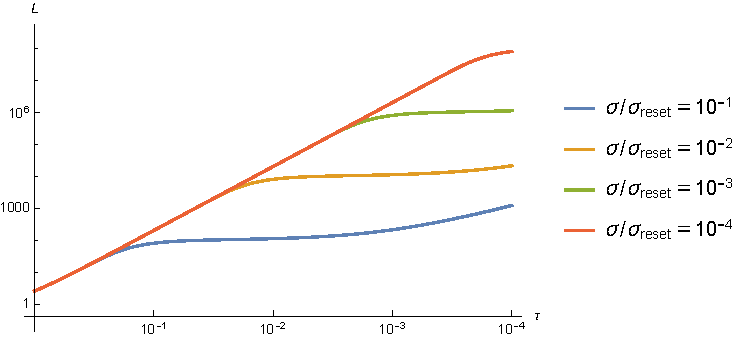
\includegraphics[width=0.7\textwidth]{reset-bf-thresholds.pdf}
    \end{center}
    \caption{
        \label{fig:reset-bf-thresholds}
        Likelihood ratio test values for various settings of the parameter
        $\tau$, and for various prior variances $\sigma / \sigma_\reset$.
        In this example, we suppose that $\mu = \mu_\reset$ and that $T_2 = 100$.
    }
\end{figure}

Importantly, this example rests on the assumption that one take a uniform
prior over whether the current prior is valid. This assumption corresponds to
that which an impartial observer might take in evaluating whether the numerical
approximations made by our rejection filter algorithm have failed for the
observed data. That is, the reset rule proposed corresponds performing an intervention
without relying on the full experimental data record. Choosing a threshold
other than $L = 1$ represents placing a different prior, as could be informed by observing
the failure modalities of many runs of the rejection filter method. As
demonstrated in \fig{reset-bf-thresholds}, because our reset rule resets with
probability 1 if a 1 is observed, choosing $\tau$ effectively sets the threshold
for $L$.
In practice,
however, because $\Pr(\text{result} = 1 | \text{prior correct}) \approx 0$, the reset
rule is only weakly dependent on the specific threshold one places on $L$.

\section{RFPE for small error tolerances}
While most of the previous data examined RFPE for relatively small error tolerances, we must examine the behavior of the algorithm for extremely
small error tolerances in order to distinguish the $O(\log(1/\epsilon))$ ideal scaling of the error versus the number of experiments and the
$O(\log(1/\epsilon)\log\log(1/\epsilon))$ scaling of Kitaev's phase estimation algorithm.  As discussed previously, we use an error correction scheme
to ensure that the inference algorithm continues to converge to the correct value inspite of surprising results which can confuse the algorithm.

We see in~\fig{small} that the error clearly follows a logarithmic scaling over this range, with no evidence of $O(\log(1/\epsilon)\log\log(1/\epsilon))$ scaling.  While we cannot formally
exclude such a scaling on theoretical grounds (owing to the heuristic nature of the algorithm), the robustness of the inference procedure over so many orders of magnitude provides
strong evidence for an $O(\log(1/\epsilon))$ scaling.


\begin{figure}[t!]
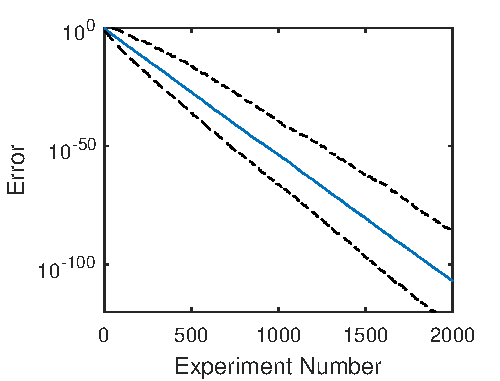
\includegraphics{longPE.pdf}
\caption{Median and $95\%$ confidence interval (dashed lines) for the error as a function of the number of experiments performed to infer an unknown phase.}\label{fig:small}
\end{figure}

%=============================================================================
\section{Time--dependent Eigenphases}
\label{app:timedep}
%=============================================================================
Another important capability that RFPE inherits from particle filter methods is the ability to track the variation of slowly changing eigenphases.
This is significant if RFPE is being used, for example, to learn an instantaneous model for a quantum device whose Hamiltonian (or control) parameters
are slowly drifting out of calibration.  By learning such drifts in an online fashion, this algorithm allows adaptive feedback to compensate for this
drift and in turn can allow the quantum device to be used even if it has substantially changed since the experimental run began.

Before continuing it is important to distinguish between two ways that time--dependent eigenphases can be examined.  The simplest approach is through hyperparameter estimation, wherein the inference process is used to learn a hyperparameter that describes the diffusion of the true eigenphase.  This can be done by introducing such a parameter into the inference problem and applying RFPE as above.  The method we favor here is different: we wish to provide an instantaneous estimate of the eigenphase.  This yields no explicit information about the extent to which eigenphases diffuse in typical cases, but it does provide the information needed to track the current value.

In principle including time--dependence in this manner is trivial since it does not require positing a dynamical model for the model parameters (unlike the hyperparameterized version).
It simply involves running RFPE without modification since ideally the algorithm should continue to track the eigenphase provided the experimental drift does not take the system beyond the 
domain of support of the prior distribution.  Such issues can be dealt with by the random restarting heuristic discussed previously.

The model of drift that we use is for drift strength $\eta$ and correlation time $\tau$, if time $M$ is taken for experiment $k$ then the eigenphase $\phi_k$ is translated according to
\begin{equation}
\phi_k \mapsto \phi_k + \eta\sqrt{M/\tau}x,
\end{equation}
where $x$ is a Gaussian random variable with zero mean and unit standard deviation.  We avoid applying the error correction method described above by updating the posterior variance given by adding in the variance introduced by the drift due to $\eta \ne 0$.

\begin{figure}
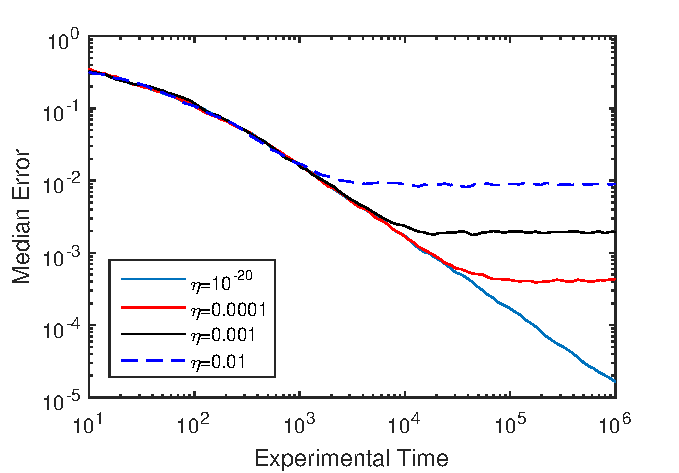
\includegraphics[width=0.6\linewidth]{Timedep.pdf}
\caption{Error in eigenphase as a function of the evolution time (the total sum of all $M$ taken for the case where $M$ is continuous) for $\tau=100$.}\label{fig:Timedep}
\end{figure}

We see in~\fig{Timedep} that the error in the unknown eigenphase does not diverge with time.  Rather, it saturates at a level that is proportional to $\eta$.  This illustrates that RFPE is capable of tracking a time dependent eigenphase, although the drift in that eigenphase places limitations on the precision of the \emph{instantaneous} estimate of the phase.

%=============================================================================
\section{Pseudocode for Algorithms}
\label{app:pseudocode}
%=============================================================================

In the main body we sketched the details of our phase estimation algorithm.  Here we elaborate on this algorithm and discuss some of the
subtle details needed to make the algorithm work.  The first such subtlety stems from the fact that eigenphases are equivalent modulo $2\pi$.  
To see this problem, consider a Gaussian distribution centered at $0$.  If we take the outputs of the distribution in the branch $[0,2\pi]$ then we find that the mean of the distribution is $\pi$ rather than $0$.  Since the support of the initial Gaussian may be small at $\phi=\pi$, such errors can be catastrophic during the inference procedure.  This can be dealt by using the circular mean and by working with a wrapped normal distribution.  This approach is discussed in~\alg{crej2}.  For expedience, we eschew this approach and instead use a heuristic approach that does  not require a large number of trigonometric calls, which can be expensive if the device performing the inference does not have native trigonometric calls.

The heuristic approach, described in~\alg{crej}, uses rejection sampling and incremental methods to estimate the mean and standard deviation of the posterior distribution.  If $\sigma\ll 2\pi$ then the probability distribution is narrow and does not suffer from significant wrap around unless $\mu \mod 2\pi \approx 0$.  We address this by keeping track of each of the accepted $\phi_j$ as well as $\phi_j+\pi$.  If $\sigma\ll 1$ than it is impossible that both distributions suffer from substantial wrap around.  The arithmetic, rather than circular, mean and standard deviation are then computed for both using an incremental formula and the branch with the smallest variance is kept.  If the branch that was shifted by $\pi$ is chosen, then $\pi$ is subtracted from the reported mean.  The standard deviation does not need to be modified because it is invariant with respect to displacements of the mean.

While this approach is correct if $\sigma\ll 1$, it is only approximate if $\sigma$ is on the order of $1$.  In such cases, computation of the circular mean is much better justified, however we find that using our heuristic approach continues to provide acceptable results while avoiding trigonometric calls that can be expensive in some contexts.  An alternative approach to solving this problem is to begin each phase estimation run with a batch of random experiments, as per~\cite{SHF14}, before continuing to ensure that the posterior variance is small enough to neglect the wrap around effect.

We give pseudocode for the reset rule that we use in practice in our numerical experiments in~\alg{restart}.  This reset rule is slightly more general than the one mentioned in the main body and includes a heuristic for detecting if the inference has made a mistake independent of whether there is decoherence in the system.  In particular, it works by performing experiments and using an estimate of the derivative of $\log(\sigma)$ to infer whether the algorithm is actually still learning.  If the derivative is too small then the algorithm resets.  Of course, a spurious result can always cause the derivative estimate to lead to a restart at a time when restarting is not advisable.  To this end, we include a counter that only resets according to this heuristic once enough data is gathered to estimate the derivative accurately.  We typically use $5$ such data points in our numerical experiments.

The choice of the evolution time and the inversion angle strongly impacts the efficiency of the learning algorithm.  We provide below code for a modified version of the
particle guess heuristic of~\cite{wiebe_hamiltonian_2014}.  As discussed in the main body, we expect that choosing $M> T_2$ will typically lead to worse estimates of the eigenphase because the effects of decoherence overwhelm the information that can be gleaned from these long experiments.  As a result, we modify the particle guess heuristic  to never choose $M> T_2$.  We formally state this procedure in~\alg{pghT2}.


\begin{figure}[h]
\begin{algorithm}[H]
    \caption{Bayes Update for \CRej using Directional Statistics}
    \label{alg:crej2}
    \begin{algorithmic}

        \Require Prior mean and variance $\mu,\sigma$, measurement $E$,
            settings $M,\theta$, number of attempts $m$, scale $\kappa_E$

        \linecomment{Initialize accumulators to 0.}
	\State $(x_{\rm inc},y_{\rm inc},N_a) \gets 0$.
%        \State{$(\mu_{\rm inc},V_{\rm inc},N_a) \gets 0$}
        \linecomment{Attempt each sample.}

        \For{$i \in 1 \to m$}
            \State $x \sim\frac{e^{-(\phi-\mu)^2/2 \sigma^2}}{\sigma\sqrt{2 \pi }},$
          
            \linecomment{Accept or reject the new sample.}
            \State $u \sim \operatorname{Uniform}(0, 1)$
            \If{$P(E | x) \ge \kappa_Eu$}% \Comment{Check if sample is accepted}
    %                \State Append $x$ to $X$.
                \linecomment{Accumulate using the accepted sample using Cartesian coordinates.}
                \State $x_{\rm inc} \gets x_{\rm inc}+ \cos(x)$
                \State $y_{\rm inc} \gets y_{\rm inc}+ \sin(x)$
                \State $N_a \gets N_a +1$.
            \EndIf
        \EndFor

        \State $x_{\rm inc}\gets x_{\rm inc}/N_a $
        \State $y_{\rm inc}\gets y_{\rm inc}/N_a $

        \linecomment{Return mean, variance of the posterior using accumulators.}
	\State $\mu\gets {\rm Arg}(x_{\rm inc}+iy_{\rm inc})$.
\linecomment{Use circular standard deviation to estimate SD for wrapped Gaussian}
	\State $\sigma = \sqrt{\ln\left(\frac{1}{\sqrt{x_{\rm inc}^2 + y_{\rm inc}^2}}\right)}$
        \State\Return $(\mu,\sigma)$

    \end{algorithmic}
\end{algorithm}
\end{figure}

% See http://tex.stackexchange.com/questions/231191/algorithm-in-revtex4-1
% for details as to why this is in a {figure} and has [H].
\begin{figure}[h]
\begin{algorithm}[H]
    \caption{Bayes Update for \CRej}
    \label{alg:crej}
    \begin{algorithmic}

        \Require Prior mean and variance $\mu,\sigma$, measurement $E$,
            settings $M,\theta$, number of attempts $m$, scale $\kappa_E$

        \linecomment{Initialize accumulators to 0.}
        \State{$(\mu_{\rm inc},\mu_{\rm inc}',V_{\rm inc},V_{\rm inc}',N_a) \gets 0$}
        \linecomment{Attempt each sample.}
        \For{$i \in 1 \to m$}
            \linecomment{Draw a sample using each ``cut'' of the prior.}
            \State $x \sim\frac{e^{-(\phi-\mu)^2/2 \sigma^2}}{\sigma\sqrt{2 \pi }},$
            \State $x\gets x \mod 2 \pi$.
            \State $x'\gets x+\pi \mod 2 \pi$.

            \linecomment{Accept or reject the new sample.}
            \State $u \sim \operatorname{Uniform}(0, 1)$
            \If{$P(E | x) \ge \kappa_Eu$}% \Comment{Check if sample is accepted}
    %                \State Append $x$ to $X$.
                \linecomment{Accumulate using the accepted sample w/ each ``cut.''}
                \State $\mu_{\rm inc} \gets \mu_{\rm inc}+ x$
                \State $V_{\rm inc} \gets V_{\rm inc}+ x^2$
                \State $V_{\rm inc}' \gets V_{\rm inc}'+ x'^2$
                \State $N_a \gets N_a +1$.
            \EndIf
        \EndFor
        \linecomment{Return mean, variance of the posterior using accumulators.}
        \State $\mu'\gets \mu_{\rm inc}/N_a $
        \State $\sigma' \gets \min\left(\sqrt{\frac{1}{N_a -1}\left(V_{\rm inc} - \mu_{\rm inc}^2 \right)},\sqrt{\frac{1}{N_a -1}\left(V_{\rm inc}' - \mu_{\rm inc}'^2 \right)}\right)$%\Comment{Use incremental formula for sample covariance}
        \State\Return $(\mu',\sigma')$

    \end{algorithmic}
\end{algorithm}
\end{figure}





\begin{figure}
\begin{algorithm}[H]
    \caption{Restarting algorithm}
    \label{alg:restart}
\begin{algorithmic}
        \Require Prior \CRej state, records of all previous models found in the phase estimation algorithm $\mu$, $\vec{\sigma}$, initial standard deviation $\sigma_{\rm init}$, $M$, $T_2$, a counter $\text{CNT}$, a maximum value of $\text{CNT}$ $\text{MAXCNT}$, $\Gamma$ and $\tau$.
	\Ensure $\text{CNT}$, $\sigma$ 
        \Function{$\text{Restart}$}{${\mu}$, $\vec \sigma$,$\sigma_{\rm init}$, $M$, $T_2$, $\text{CNT}$, $\text{MAXCNT}$, $\Gamma$, $\tau$}
	\State $D \gets$ derivative of $\log{\sigma}$.
	\If {($D\ge \Gamma$ and $\text{CNT}\ge {\rm MAXCNT}$) or rand()$>\exp(-M/T_2)$}\Comment{Checks to see if the eigenstate is suspect.}
		\State Perform experiment with $M=\tau/\sigma$ and $\theta=\mu$.
		\If{Outcome is 0}\Comment{Test concludes state estimate is valid}
\State ${\rm CNT} \gets {\rm CNT}+1$.
			
\Else\Comment{Test concludes state estimate is invalid}

		

\State $\text{CNT}\gets 0$
	\State $\sigma \gets \sigma_{\rm init}$
	%\State \Return $\text{CNT}, \sigma$
\EndIf
\Else\Comment{Does not restart if state is not suspect}
	\State $\text{CNT}\gets \text{CNT}+1$
	%	\State \Return $\text{CNT},\sigma$.
	\EndIf
\State \Return $\text{CNT},\sigma$.
        \EndFunction
    \end{algorithmic}
\end{algorithm}
\end{figure}


\begin{figure}
\begin{algorithm}[H]
    \caption{PGH for decoherent phase estimation using \CRej}
    \label{alg:pghT2}
\begin{algorithmic}
        \Require Prior \CRej state $\mu$, $\Sigma$. Resampling kernel $\operatorname{F}$.
        \Ensure  An experiment $(M, \theta)$.
        \Function{$\text{PGH}_\text{\CRej}$}{$\mu$, $\Sigma$, $T_2$}
            \State $M \gets 1.25 / \sqrt{{\rm Tr}(\Sigma)}$
    \If {$M\ge T_2$}
        \State $M\sim f(x;1/T_2)$\Comment{Draw $M$ from an exponential distribution with mean $T_2$}.
    \EndIf
            \State $(-\theta/M) \sim \operatorname{F}(\mu, \Sigma)$
            \State \Return $(M, \theta)$.
        \EndFunction
    \end{algorithmic}
\end{algorithm}
\end{figure}

%=====================================================================
\bibliographystyle{apsrev}
\bibliography{CRPE}
%=====================================================================

\end{document}